\subsection{Punto de Vista: Descripción del problema.}

\subsubsection{Punto de Vista: Contexto de la solución (Diagrama de Contexto)}


\subsection{Punto de Vista: Interacción}
El punto de vista de interacción tiene como propósito representar cómo los diferentes actores del sistema ChibchaWeb se comunican con los componentes funcionales durante la ejecución de casos de uso específicos.

\subsubsection{Diagrama de Casos de Uso}

Muestra la interacción entre los actores principales del sistema ChibchaWeb y los casos de uso que pueden ejecutar. Esta vista representa la funcionalidad del sistema desde el punto de vista de cada actor y su relación directa con los servicios ofrecidos, recalcar que aunque igual son numeros diagramas se intento ser lo más especifico en las funcionalidades planteadas para el proyecto, las funcionalidades de valor agregado al proyecto no fueron incluidas tales como buscar dominio por IA o el chatbot, el diagrama completo se encontrara en la sección de anexos.

\subsubsection{Diagramas de Secuencia}

Los diagramas de secuencia representan la dinámica del sistema durante la ejecución de casos de uso específicos. En ellos se detalla el orden cronológico de los mensajes intercambiados entre los actores y los objetos o componentes internos del sistema, todos estos diagramas se encontraran en la sección de anexos.\\

Esto Nos Permite Ver:

\begin{itemize}
\item Cómo se coordinan los distintos elementos para cumplir una funcionalidad.

\item Qué actores o servicios están involucrados.

\item Cómo fluye la lógica de negocio a través de las capas del sistema.
\end{itemize}


\subsubsection*{1. Agregar Método De Pago}

Este diagrama de secuencia representa el proceso mediante el cual un cliente registra un nuevo método de pago (tarjeta de crédito o débito) en la plataforma ChibchaWeb. El proceso inicia cuando el cliente ingresa los datos de su tarjeta en el formulario correspondiente.

El sistema separa internamente el flujo en dos pasos:

\begin{enumerate}
    \item Primero se realiza una llamada a la API /tarjeta para registrar los datos de la tarjeta en la base de datos.
    \item Luego, se ejecuta la llamada a /MetodoDePagopara asociar el método de pago a la cuenta del cliente.
\end{enumerate}

Ambas solicitudes son gestionadas por el módulo encargado de manejar los métodos de pago. Una vez completadas las operaciones en la base de datos, el sistema confirma al cliente que el método fue agregado correctamente.

\subsubsection*{2.  Registrarse Como Distribuidor}

Este diagrama de secuencia ilustra el proceso completo de registro de un nuevo distribuidor en la plataforma ChibchaWeb. El flujo inicia cuando el usuario llena el formulario de registro con su información personal y empresarial.

Una vez enviado el formulario:

\begin{enumerate}
\item El controlador de registros valida y procesa los datos recibidos.

\item Se genera una nueva cuenta en la base de datos del sistema.

\item Simultáneamente, el sistema genera un token de verificación y lo envía al correo electrónico del distribuidor mediante el servicio de correo.
\end{enumerate}

El distribuidor recibe un mensaje en pantalla indicando que debe verificar su cuenta para completar el proceso de registro y poder acceder al sistema con normalidad.

\subsubsection*{3. Registrarse Como Cliente}

Este diagrama de secuencia describe el proceso mediante el cual un cliente se registra en la plataforma ChibchaWeb. El flujo comienza cuando el cliente llena el formulario de registro desde el frontend.

El sistema ejecuta los siguientes pasos:

\begin{enumerate}
    \item La información del formulario es enviada a la API de registro.
    \item La API delega la validación de los datos a un servicio de validación.
    \item Una vez validados los campos, la API crea una nueva cuenta en la base de datos.
    \item Posteriormente, se genera un token de verificación a través del servicio de tokens, el cual es almacenado nuevamente en la base de datos.
    \item Finalmente, se utiliza el servicio de correo para enviar el mensaje de verificación al correo del cliente.
\end{enumerate}

El proceso concluye mostrando un mensaje al usuario con la instrucción de verificar su cuenta.

\subsubsection*{4. Generar archivo de dominio}

Este diagrama de secuencia representa el proceso completo mediante el cual un usuario envía una solicitud para registrar un dominio a través de la plataforma ChibchaWeb. El flujo incluye desde el ingreso inicial de los datos hasta la generación y envío del archivo XML al registrador externo.

El proceso sigue los siguientes pasos:

\begin{enumerate}
\item El usuario llena el formulario y envía la solicitud.
\item El controlador de dominio envía los datos al servicio de dominio, que los procesa y gestiona.
\item La solicitud se guarda a través del backend API, que la inserta en la base de datos y recibe un identificador.
\item Luego, se genera un archivo XML con los datos de la solicitud.
\item El archivo generado es enviado al registrador externo.
\item Tras la confirmación del registrador, se actualiza el estado de la solicitud en el sistema.
\item Finalmente, se muestra al usuario un mensaje confirmando que la solicitud fue enviada correctamente.
\end{enumerate}

\subsubsection*{5. Cargar Pagos a Tarjeta}
Este diagrama de secuencia muestra el proceso que se ejecuta cuando un cliente confirma la compra de un servicio desde el carrito, utilizando una tarjeta previamente registrada como método de pago.

El flujo se desarrolla de la siguiente forma:

 \begin{enumerate}
 \item El cliente confirma la compra desde el frontend, lo que activa el controlador de pagos.
 \item El controlador de pago solicita al backend API la verificación del método de pago seleccionado.
 \item El backend consulta la base de datos para validar la tarjeta asociada y, si es válida, procede a procesar la transacción con el servicio de pago externo.
 \item El servicio responde si el resultado fue aprobado o rechazado.
 \item En caso de aprobación:
 \begin{enumerate}
     \item Se confirma el pago del carrito.
     \item Se actualiza el estado del carrito en la base de datos.
     \item El cliente recibe un mensaje confirmando el éxito de la operación.
 \end{enumerate}

 \item Si el pago es rechazado:
    \begin{enumerate}
    	\item El sistema muestra un mensaje de error indicando que la transacción fue fallida.
    \end{enumerate}
 \end{enumerate}

\subsubsection*{6. Registrar Solicitud De Dominio}

Este diagrama de secuencia representa el flujo de interacción cuando un usuario desea registrar un dominio a través del sistema ChibchaWeb. La funcionalidad incluye una validación previa en tiempo real para comprobar si el nombre de dominio está disponible.

El proceso se detalla a continuación:

\begin{enumerate}
    \item El usuario ingresa el nombre del dominio en el formulario de registro.
    \item El controlador de registro de dominio consulta la disponibilidad del dominio utilizando un servicio de scraping, el cual accede a un registrador externo.
    \item Si el dominio está disponible:
    \begin{enumerate}
        \item Se realiza una solicitud POST para registrar el dominio a través del backend API.
        \item Esta solicitud se guarda en la base de datos, y se actualiza el estado del dominio como ocupado.
        \item El sistema muestra un mensaje indicando que la solicitud fue registrada exitosamente.
    \end{enumerate}

    \item Si el dominio no está disponible:
    \begin{enumerate}
    	\item Se muestra un mensaje de error al usuario indicando que el dominio ya está ocupado.
    \end{enumerate}
\end{enumerate}

\subsubsection*{7.Gestionar Perfiles De Clientes/Empleado}

Este diagrama de secuencia representa el proceso mediante el cual un distribuidor puede buscar, editar o eliminar perfiles de clientes en la plataforma.

El flujo incluye:

\begin{itemize}
    \item Búsqueda: El distribuidor consulta un cliente. El sistema recupera los datos desde la base de datos y los muestra en la interfaz.

    \item Edición: Se modifican los datos del perfil. La información se actualiza en la base de datos y se notifica al distribuidor.

    \item Eliminación: Se confirma la eliminación del perfil, la base de datos ejecuta la operación y se devuelve una respuesta de confirmación.
\end{itemize}

\subsubsection*{8. Calcular Comisión De Distribuidores}

Este diagrama de secuencia representa el proceso mediante el cual un administrador ejecuta el cálculo de comisiones para distribuidores en función de sus ventas registradas.

El flujo general es el siguiente:

\begin{enumerate}
    \item El administrador inicia el proceso desde la vista administrativa.
    \item El controlador de comisiones solicita al servicio de comisiones la ejecución del cálculo.
    \item Se consultan en la base de datos las ventas asociadas a cada distribuidor.
    \item El sistema aplica el porcentaje de comisión correspondiente ($10\% $ para distribuidores BÁSICOS y $15\%$ para PREMIUM).
\end{enumerate}

\subsubsection*{9. Generar Transferencia}

Este diagrama de secuencia describe el proceso mediante el cual un cliente transfiere la propiedad de un dominio a otro usuario de la plataforma, utilizando su dirección de correo como identificador.

El flujo se compone de los siguientes pasos:

\begin{enumerate}
    \item El cliente ingresa el dominio a transferir y el correo de destino en la interfaz correspondiente.
    \item El controlador de transferencia gestiona la solicitud y la envía al API de transferencia.
    \item El backend consulta la base de datos para verificar que la cuenta de destino existe y que el dominio pertenece al cliente actual.
    \item Si todo es válido, se actualiza el propietario del dominio en la base de datos.
    \item Finalmente, se muestra al cliente un mensaje indicando que la transferencia fue exitosa.
\end{enumerate}

\subsubsection*{10. Registrar Empleado}

 Este diagrama muestra el proceso mediante el cual un administrador registra un nuevo empleado en la plataforma ChibchaWeb.

El flujo sigue los siguientes pasos:

\begin{enumerate}
    \item El administrador completa el formulario de registro desde la vista administrativa.
    \item El controlador de registro de empleados recibe los datos y realiza una solicitud POST a la API de registro.
    \item La API almacena la información en la base de datos y devuelve una confirmación.
    \item Finalmente, el sistema muestra un mensaje notificando que el empleado fue registrado exitosamente.
\end{enumerate}

\subsubsection*{11. Registrar Tickets}

Este diagrama de secuencia representa el proceso mediante el cual un usuario crea un ticket de soporte en la plataforma ChibchaWeb, detallando un asunto y una descripción del problema.

El flujo es el siguiente:

\begin{enumerate}
    \item El usuario completa el formulario de soporte con los datos requeridos.
    \item El controlador de tickets procesa la solicitud y la envía mediante una petición POST a la API de creación de tickets.
    \item La API almacena el ticket en la base de datos y genera un identificador único.
    \item Finalmente, se muestra al usuario un mensaje de confirmación indicando que el ticket fue creado correctamente.
\end{enumerate}

\subsubsection*{12. Consultar Tickets}
Este diagrama de secuencia describe el proceso en el cual un usuario (cliente, distribuidor, empleado o soporte) accede al módulo de soporte técnico para consultar los tickets que le han sido asignados o que ha creado previamente.

El flujo contempla dos variantes según el tipo de usuario:

\begin{enumerate}
    \item Si el usuario es cliente o distribuidor, se realiza una solicitud GET /consultarTicketporIDCUENTA.
    \item Si es empleado o soporte técnico, se usa GET /mis-tickets-empleado.
\end{enumerate}

En ambos casos:

\begin{itemize}
    \item La solicitud es gestionada por el controlador, que la envía a la API de tickets.
    \item La API consulta la base de datos y devuelve la lista de tickets encontrados.
    \item Finalmente, la lista se muestra al usuario en la interfaz.
\end{itemize}

\subsubsection*{13. Atender Y Escalar Tickets}

Este diagrama de secuencia ilustra el proceso que realiza un usuario del área de soporte técnico para visualizar sus tickets asignados, actualizar su estado (por ejemplo, de "pendiente" a "en proceso" o "resuelto") y, si corresponde, escalar el ticket a un nivel superior.

El flujo incluye dos acciones principales:

\begin{enumerate}
\item \textbf{Atender Ticket (Cambiar Estado):}
\begin{itemize}
    \item El soporte accede al panel donde visualiza sus tickets.
    \item A través del controlador, el sistema obtiene los tickets desde la API y los recupera de la base de datos.
    \item El soporte selecciona un ticket y un nuevo estado, lo cual genera una solicitud PATCH /CambiarEstadoTicket.
    \item El estado se actualiza en la base de datos y se notifica al usuario.
\end{itemize}

\item \textbf{Escalar Ticket:}
\begin{itemize}
\item Si el ticket requiere mayor atención, el soporte ejecuta una acción para escalarlo.
\item Se envía una solicitud PATCH /CambiarNivelTicket con el identificador del ticket.
\item El backend registra el cambio de nivel, actualizando la información del ticket y notificando al usuario que el ticket fue escalado.
\end{itemize}
\end{enumerate}

\subsubsection*{14. Iniciar Sesión}

Este diagrama de secuencia describe el proceso de inicio de sesión en la plataforma ChibchaWeb por parte de un usuario, contemplando tres posibles resultados: acceso completo, acceso limitado (por cuenta no verificada) o error por credenciales inválidas.

El flujo es el siguiente:

\begin{enumerate}
\item El usuario ingresa sus credenciales en la vista de login.
\item El controlador de login las envía a la API, que consulta la base de datos para verificar:
\begin{itemize}
    \item La existencia del usuario.
    \item Que la contraseña coincida.
    \item Si la cuenta está verificada.
\end{itemize}

\item Si las credenciales son válidas:
\begin{enumerate}
    \item Si la cuenta está verificada: se inicia sesión, se devuelve un token y se redirige según el rol.
    \item Si no está verificada: se limita el acceso y se notifica al usuario que debe verificar su cuenta.
\end{enumerate}

\item Si las credenciales son inválidas:
\begin{enumerate}
	\item Se muestra un mensaje de error indicando el fallo.
\end{enumerate}
\end{enumerate}

\subsubsection*{15.Buscar Cuenta}

Este diagrama de secuencia muestra el proceso que sigue un administrador para consultar la información de una cuenta existente, utilizando como criterio de búsqueda un correo electrónico o ID.

El flujo es el siguiente:

\begin{enumerate}
    \item El administrador ingresa el correo o identificador en la vista de administración.
    \item El controlador de búsqueda de cuentas envía la solicitud al endpoint correspondiente de la API.
    \item La API consulta la base de datos para recuperar los datos de la cuenta asociada.
    \item Una vez encontrada, se retorna la información del perfil y se presenta al administrador.
\end{enumerate}

\subsubsection*{16. }

Este diagrama de secuencia describe el proceso mediante el cual un usuario accede a la sección “Mi Perfil” dentro de la plataforma ChibchaWeb para visualizar su información personal.

El flujo incluye los siguientes pasos:

\begin{enumerate}
\item El usuario navega a la vista de perfil desde la interfaz.
\item El controlador de perfil realiza una solicitud POST al endpoint /cuenta\_por\_correo en la API, pasando el identificador del usuario.
\item La API consulta la base de datos para obtener los datos asociados al correo.
\item Los datos del perfil (como nombre, correo, dirección, etc.) son devueltos y mostrados en pantalla.
\end{enumerate}

\subsubsection*{17. Validar Datos}

Este diagrama de secuencia describe el proceso de validación de datos ingresados por un usuario en formularios del sistema ChibchaWeb. Este flujo es común en procesos como registro, adición de tarjetas o dominios, y garantiza que la información ingresada cumpla con formato y disponibilidad antes de ser procesada.

El flujo contempla dos escenarios:

\begin{enumerate}
    \item \textbf{Datos válidos:}
    \begin{enumerate}
        \item El usuario ingresa los datos en el formulario.
        \item El frontend los envía al controlador de validación, que verifica el formato y la disponibilidad en la base de datos.
        \item Si no hay errores, se devuelve una respuesta confirmando que los datos fueron validados correctamente.
    \end{enumerate}

    \item \textbf{Datos inválidos o duplicados:}
    \begin{enumerate}
    	\item En caso de errores de formato o duplicidad (por ejemplo, correo o dominio ya registrados), el sistema responde con una lista de errores que se muestran al usuario.
    \end{enumerate}
\end{enumerate}

\subsection{Punto de Vista: Desarrollo}
\begin{figure}[H]
	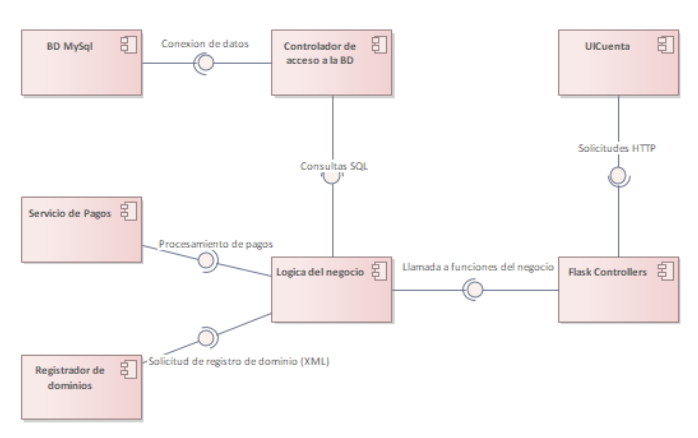
\includegraphics[width=\columnwidth]{puntovista/diacomponentes.png}
	\caption{Diagrama de componentes}
	\label{fig:diacomponentes}
\end{figure}

\subsection{Punto de Vista: Modelo Relacional de la BBDD}
